\section{Prototyping} \label{sec:Experimentation}

% Intro
We have prototyped the wireless sensors and actuator's network of traffic lights and roads on a mockup \footnote{https://github.com/IoT-UTLC/Resources/wiki} of real intersection in Paris with a scale of 1:68.
Our specifications have been defined considering the low-cost and energy efficiency of the solution.
This Testbed is a proof of concept of not limited to our use case as it is scalable for other applications.
For example,
	additional sensors of fine particules could be implanted bringing correlation between traffic jam and pollution.

\begin{figure*}[!htb]
\centering
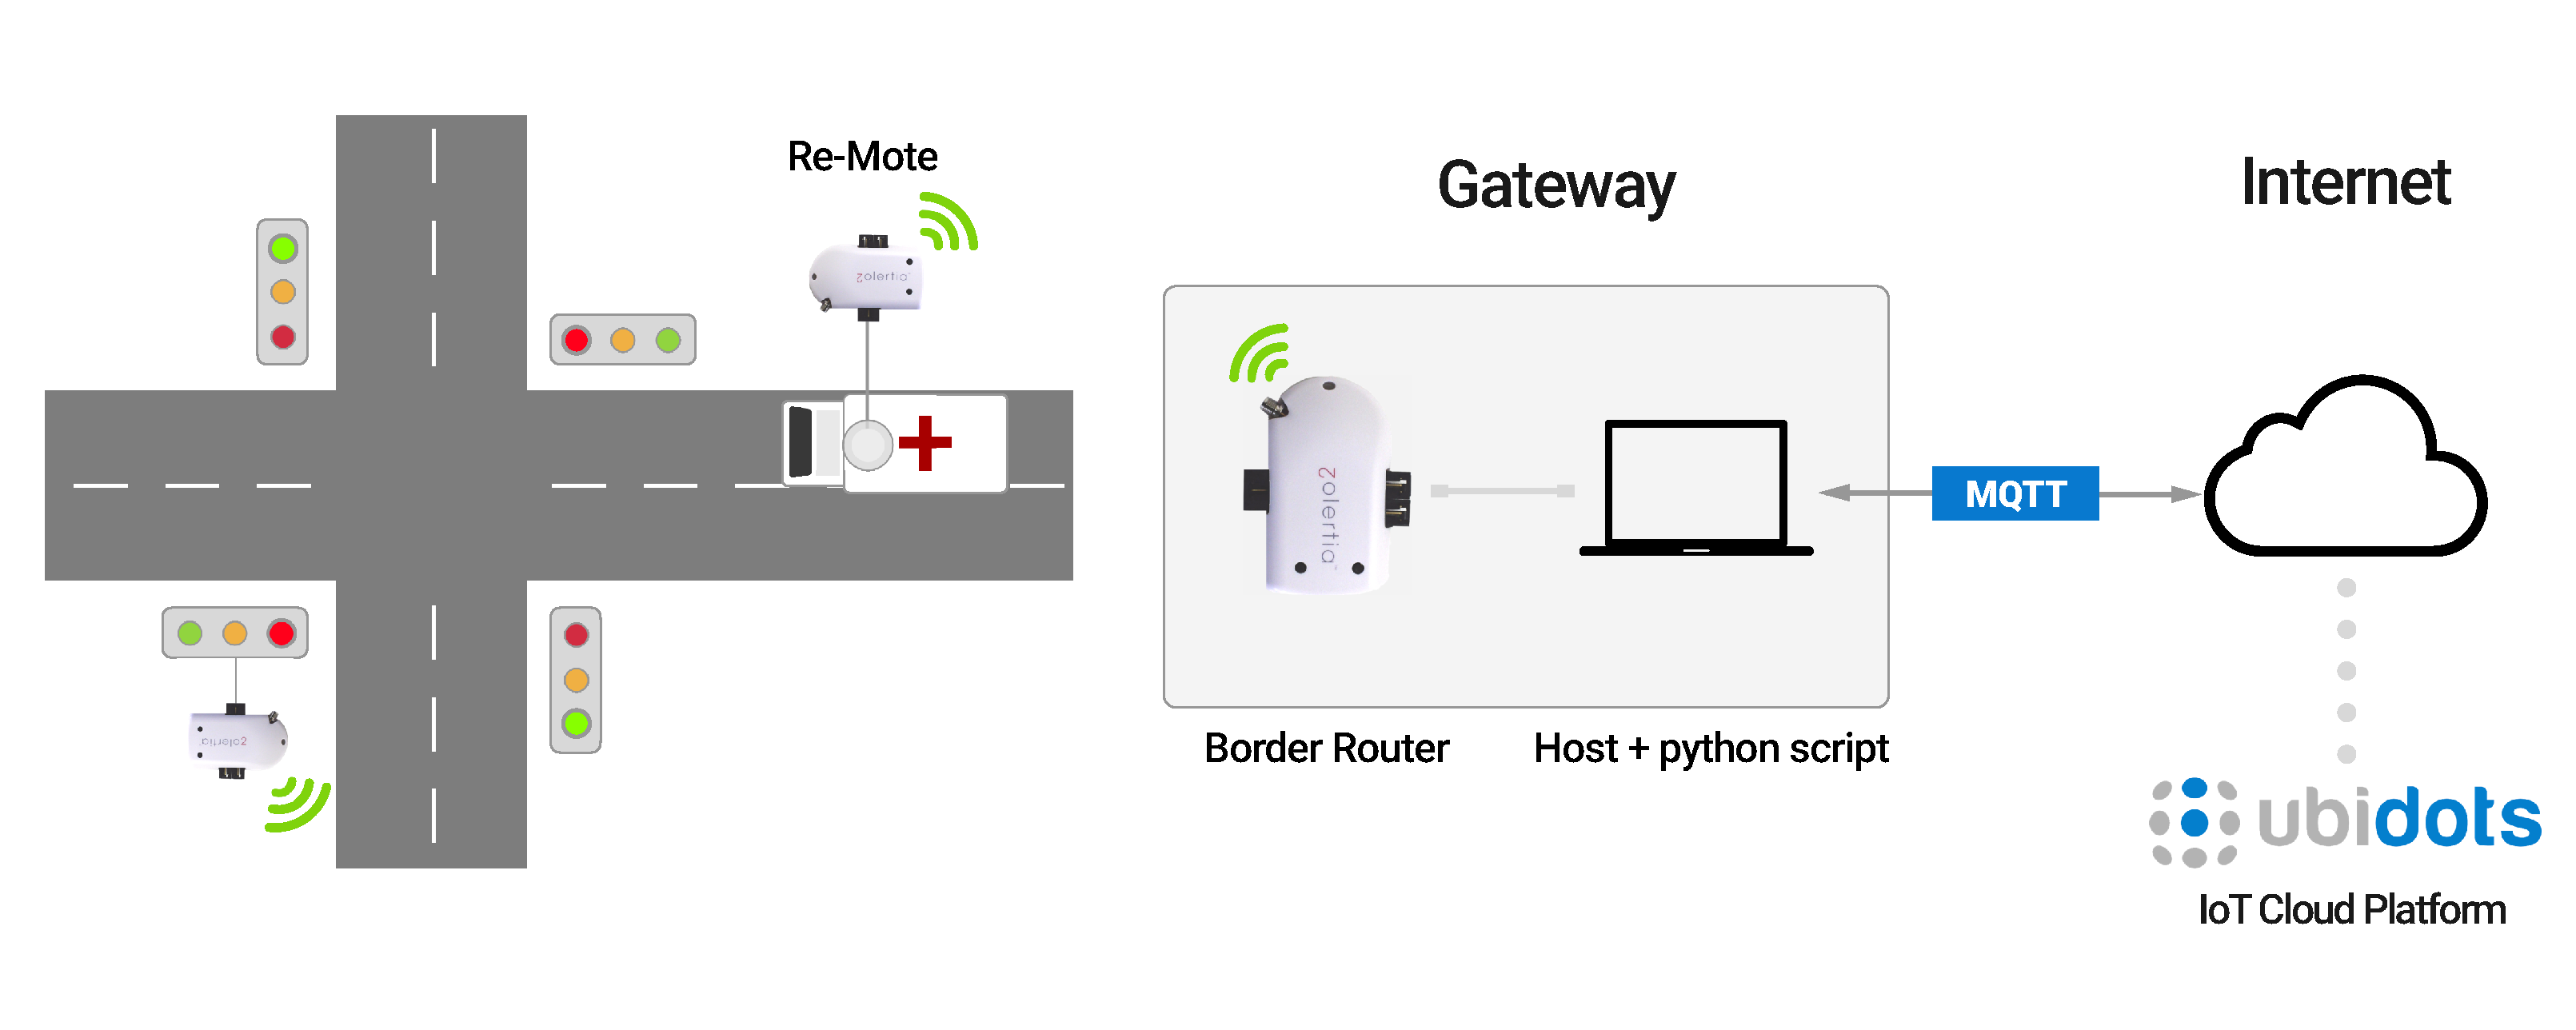
\includegraphics[width=4.5in]{Figures/ScenarioPaper.eps}
\caption{Architecture of  Iot-UTLC}
\label{fig:ScenarioPaper.eps}
\end{figure*}

Fig.
\ref{fig:ScenarioPaper.eps} shows the architecture of our IoT-UTLC with three layers.
From left to right,
	we have the WSN layer with connected traffic lights’ actuators,
	sensors and IEEE 802.15.4 transceivers.
The second part is the gateway of the WSN ensured by the BR and the Middleware \emph{i.e.} Python script launched by host computer.
The last layer is the Ubidots IoT Cloud Platform.
It is an open source solution used to collect and analyze WSN data.

\subsection{6LoWPAN, Contiki OS, Re-Mote and Border Router} \label{Sec:Contiki}

% 6LoWPAN
Our WSN is an IPv6 LowPower Wireless Personal Area Network (6LoWPAN) based on IEEE 802.15.4 stack.
It is well adapted to embedded wireless devices with energy aware constraint and for its capabilities to define a mesh topology.
Contiki Os\footnote{http://www.contiki-os.org/} has been used to implement networks' functions such as send,
	receive and data processing.
It is an embedded operating system with large open source community.
It supports Zolertia's Re-Motes \footnote{https://github.com/Zolertia/Resources/wiki/RE-Mote} and implements recent IEEE 802.15.4 standard specifications.
It also includes protocols such as RPL,
	CoAP and MQTT.
Furthermore,
	developer community is active and makes available source codes examples in order to help developing quickly new applications.

% Re-motes
Re-motes are compatible with our WSN specifications and our design model.
They are wireless devices with ultra-low power operation mode.
This choice has been motivated by long radio range of its IEEE 802.15.4 CC1200 transceiver,
	which transmits in the frequency band of 868-915 MHz.
In addition,
	each Re-Mote has analog and digital ports with a possibility to connect several analog sensors and actuators.
A Re-mote can be driven by a computer and become a sink and/or BR as well as a gateway between the 6LoWPAN network and the computer.

%\Figure{!htb}{1}{ethernetRouter.png}{Our Ethernet router}
\begin{figure}[!htb]
\centering
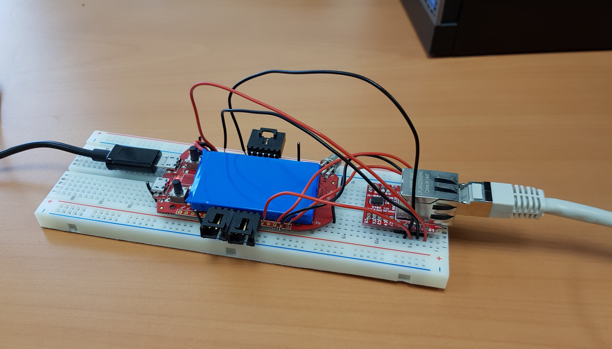
\includegraphics[width=2.5in]{Figures/ethernetRouter.png}
\caption{BR and sink combined on one board}
\label{fig:ethernetRouter.png}
\end{figure}

%[Explanation of how it works with the 2 radios,
To implement the previous model described in Section \ref{sec:Use Case and Model Design},
	we used six Re-motes:
	one for the BR,
	four to control the traffic lights and one Re-Mote to detect the arrival of a high priority vehicle near a crossing point.
For simplicity,
	we choose a touch sensor as a detecting device of priority vehicle.
We have developed four types of programs running on a Re-mote:
	traffic lights signs,
	sensors,
	high priority vehicle detecting device and BR function.
Sensors send periodically information to the IoT Cloud Platform with temperature,
	pressure or any relevant information that can be sensed.
As mentioned in the previous section,
	traffic lights are sub-divided into two modes:
	slaves and masters.
Masters nodes are the only ones to request the Middleware to change its light’s state and slaves simply change its state depending on received packets.
These roles are defined to reduce the overhead of network,
	redundancy and collisions,
	for instance.
Masters send periodically packets to request a change of state to the Middleware which forwards them to a Cloud platform.
 
BR node behaves differently compared to the other Re-motes.
The entries of its routing table are the list of Re-motes that pass through it.
It reroutes every packet it receives from its neighboring to host computer (or sink),
	which  creates a connection to the IoT Cloud platform.
Two options are possible to create our BR:
	i) separate the BR and sink and ii) combine both on the same device.
In our development,
	we worked on how to implement the sink and the BR nodes on the same Re-Mote board.
Fig.
\ref{fig:ethernetRouter.png} shows a prototype of the combined BR and sink,
	both connected to an ethernet interface.
Indeed,
	if the border router becomes an Ethernet router,
	there will no longer be any connection between the host/sink machine and the IoT Cloud platform.
Every Re-mote is able to connect independently to the IoT Cloud platform.
This approach has some advantages,
	such as the autonomy of the devices,
	but it generates an overhead requiring extra synchronization packets' exchange.
Therefore,
	we separate the sink and BR,
	since this solution is more flexible and resilient for our Testbed.

%The border router is at first a Re-mote,
%	but it has very different behavior and function.
%Indeed it has the task of re-routing every packet it receives from its cohorts to the serial port of the host machine.


%This machine will create a connection to the IoT Cloud platform and send the Re-motes messages to it and get responses for the Re-motes.
%The border router is a central node because it knows all to Re-motes in the 6LoWPAN which packets have transited by it.
%It acts as a Router and has a routing table of those Re-motes that pass through it.
%A web server page can be accessed to retrieve that information.
%We also tried a different approach of it.

 % [
%Transition with next paragraph => the use of MQTT to access the other "side" of the system
%Explanation of how it works (encapsulating the headers ...)
%]
%[
%Big part of how it works,
%what is good about it %New paragraph about the autonomous BR we were trying to develop
%Comparison between the 2 solutions
%]

% Autonomous BR
%As we have seen before,
%	this approach requires a Border Router linked the computer itself to the internet,
%	we tried to see if we can remove one part.
%Thus,
%	we added a component to the Re-mote in order to connect it directly to the internet via an Ethernet cable.

%[Transition with next paragraph => the use of MQTT to access the other "side" of the system]

\subsection{MQTT and UBIDOTS} \label{Sec:MQTT}

Fig.
\ref{fig:StackIoT.pdf} presents the layers of our UTLC network.
From bottom to up,
	the WSN network sense and/or detect,
	process and actuates traffic lights.
The second layer manages the 6 LowPan addressing and routing of packets throughout an IEEE 802.15.4 network.
The Edge Computing is the Middleware between the WSN and the Cloud platform.
For the setup of our UTLC,
	we start by establishing the access network of WSN.
The next step is to connect this network to Core network.
MQTT protocol controls three levels of QoS of exchanged packets from the WSN to the chosen Ubidots \footnote{https://ubidots.com/} Cloud platform.
It adopts IntServ approach for supporting quality of service in the network,
	it tags incoming packets in the border routers with different levels of priority.
Core routers read incoming packets headers and queue them according to their priority,
	packets with a high priority are sent faster compared to low priority ones.

MQTT ensures the QoS and publish/subscribe mechanisms through a broker.
The broker behaves as a server by filtering messages and organizing them in topics,
	which are strings used to filter messages and define the hierarchy of our data structure.
They allow us to organize how to receive multiple data from sensors such as temperature,
	up time,
	battery status and how to display them and obtain a real-time glance of our system.
It gets its messages from publishers and sends any modifications to entities,
	which that subscribed to the updated topics.
We used this mechanism with the Middleware in order to publish messages to the broker and get from the main topic the new values of the subscriber.

%We have seen in previous section what we used for our local sensors network, let's see now how we communicate with the IoT Cloud Platform. We will use MQTT which is a light-weight transportation protocol. In our solution, a python script will run an MQTT client to connect our WSN to Ubidots.

%MQTT ensures the QoS and publishes/subscribes mechanisms with a noteworthy topic organization. 

%The topics are strings used to filter messages and define the hierarchy of our data structure. They allow us to organize how to receive multiple data from sensors such as temperature, up time, battery status and how to display them and obtain a real-time glance of our system. 

%In addition, the broker behaves as a server by filtering messages and organize them in topics. It gets its messages from publishers and will send any modifications to entities which would have subscribed to the updated topics. We used this mechanism with the middleware in order to publish messages to the broker and get from the main topic the new values using the subscriber functionality.


The QoS feature of MQTT protocol manages network resources by handling retransmissions and guarantees the delivery of messages. It allows more control on messages by defining the level of guarantee. By default, the QoS is defined by three levels. The first one, level 0, is `At most one`. Level 1 is `At least one` where there is an acknowledgment to let the sender know that its packet has been received. Finally, level 2 `Exactly once` is the highest verification level with a request/response flows to ensure that only one message will be delivered and processed by the receiver. In our case, we applied levels 1 and 2 using \textit{paho.mqtt.client} Python library.  
%
%For example, subscribed clients could define the data QoS level of requested data by the source code shown bellow. 
For example, publisher of high priority data such as touch sensor has to indicate the highest level of QoS by the code shown bellow. 
We shared our implementation and its source codes at https://github.com/IoT-UTLC/contiki.
%
%\begin{footnotesize}
%\begin{lstlisting}
%# client receives a CONNACK response 
%# from the server.
%def on_connect(client, userdata, flags, rc):
%  print("Subscribed to " + MQTT_URL_TOPIC)
%  client.subscribe(MQTT_URL_TOPIC, 2) 
%  # 2nd arg is the QoS level to use 
%  # at maximum when it's needed
%\end{lstlisting}
%\end{footnotesize}

\begin{footnotesize}
\begin{lstlisting}
payload = json.dumps({"RoadA": data, "RoadB": 0})
res, mid = conn.publish(MQTT_URL_PUB, payload,
	  qos=int(QoS)) # QoS is QoS level to use 
\end{lstlisting}
\end{footnotesize}


%# The callback for when the client receives a CONNACK response from the server.
%def on_connect(client, userdata, flags, rc):
%	print("Connected with result code "+str(rc))
%	print("Subscribed to " + MQTT_URL_TOPIC)
%	client.subscribe(MQTT_URL_TOPIC, 2) 
                                                                                                                                                        
We experienced significant latency of high priority messages when we tested of IoT-UTLC mockup. Therefore, assessments of the MQTT protocol in our case provided significant information about its efficiency. 

%  For the end point the IoT Cloud platform,
% we wanted to be simple  %QoS and MQTT resilient by default (good implementation)
% Get relevant information from dashboard
% Access from anywhere (remote control possible)
% Structure our system / hierarchy
%
%As for the MQTT broker, we wanted an easy and powerful IoT Cloud Platform.
%It will be compatible with all technologies we chose for our prototyping,
%	so with an integration of MQTT and QoS levels.
%an IoT Cloud platform is a central point of the system as it keeps all the information about our WSN.
%Using the Cloud allows the system being accessible from anywhere on the internet.
%It is also a tool to filter and display relevant information in real-time from our system in the centralized dashboard.
%It can be possible to trigger some actions on the system via the dashboard.
%
%% Architecture
%Building this virtual infrastructure for this project has been challenging.
%we used MQTT topics mechanism to get the most of Ubidots to structure every data sent.
%We have a main topic which contains the states of the traffic light (RoadA and RoadB) in real time,
%	we created individual topics for every Re-mote acting as traffic lights or sensors.
%With this architecture,
%	we can have deep information on every device (such as its battery,
%	sensors data,
%	etc...).
%Moreover,
%	it could be scaled to match future needs.


%\Figure{!htb}{1}{cdf_distribution.pdf}{Normal,Gamma and Logistic distribution}
\begin{figure}[!htb]
\centering
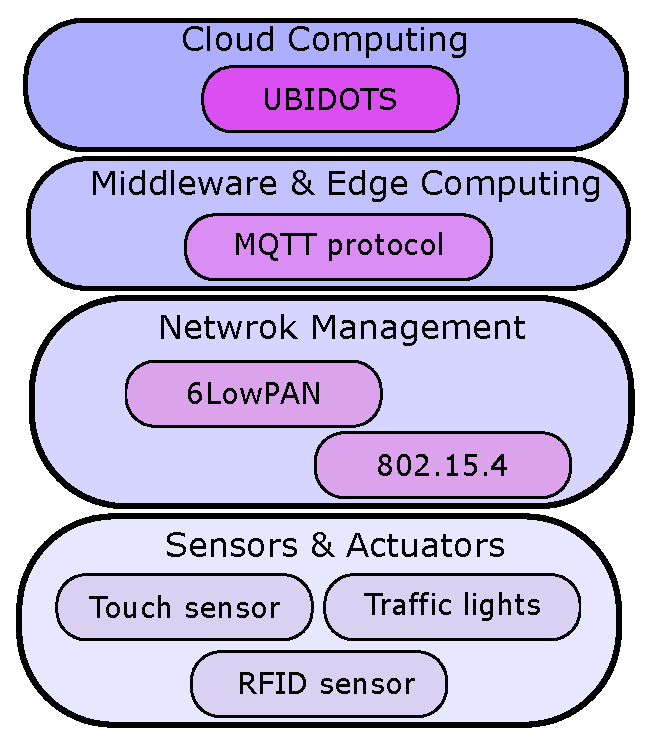
\includegraphics[width=2in]{Figures/StackIoTv1.eps}
\caption{UTLC network layers}
\label{fig:StackIoT.pdf}
\end{figure}
